% Build the projection and speaker views with make -C talk.
\documentclass[aspectratio=169,12pt]{beamer}
\usepackage{tikz,standalone,booktabs,array}
\usepackage{libertinus}
\usepackage{amsmath}
\usetikzlibrary{
  arrows.meta,
  backgrounds,
  calc,
  decorations.markings,
  fit,
  positioning
}

\definecolor{accent}{RGB}{38,103,115}
\definecolor{softgray}{RGB}{244,245,246}
\definecolor{midgray}{RGB}{123,128,132}

\tikzset{
  >={Latex[length=2.2mm,width=1.5mm]},
  flow/.style={-Latex,semithick,draw=black!72},
  accent flow/.style={-Latex,semithick,draw=accent},
  box/.style={
    draw=black!68,
    fill=softgray,
    rounded corners=1.2pt,
    align=center,
    inner xsep=5pt,
    inner ysep=4pt
  },
  accent box/.style={
    draw=accent,
    fill=accent!8,
    rounded corners=1.2pt,
    align=center,
    inner xsep=5pt,
    inner ysep=4pt
  },
  point/.style={circle,draw=black!75,fill=white,inner sep=1.7pt},
  accent point/.style={circle,draw=accent,fill=accent!10,inner sep=1.7pt},
  tinylabel/.style={font=\scriptsize,align=center},
  smalllabel/.style={font=\small,align=center},
  panel/.style={draw=black!28,rounded corners=2pt,inner sep=6pt}
}

\usefonttheme{professionalfonts}
\usefonttheme{serif}
\makeatletter
\def\input@path{{../thesis/}}
\makeatother
% Replace every placeholder before producing a submission PDF.
% The review draft shows the confirmed author and actual review-build date.
\newif\ifReviewDraft
\ReviewDrafttrue
\newcommand{\ReviewDraftDate}{20 November 2026}
\newcommand{\ThesisTitle}{Implementation and Evaluation of the 1990 Simplified Jordan Sorting Algorithm}
\newcommand{\ThesisAuthor}{Yixue Wang}
\newcommand{\MatriculationNumber}{Matriculation Number}
\newcommand{\ThesisType}{Master's Thesis}
\newcommand{\ThesisSupervisor}{Supervisor Name}
\newcommand{\SecondExaminer}{Second Examiner Name}
\newcommand{\SubmissionDate}{Submission Date}

\newcommand{\UniversityName}{Freie Universit\"at Berlin}
\newcommand{\DepartmentName}{Department of Mathematics and Computer Science}
\newcommand{\InstituteName}{Institute of Computer Science}
\newcommand{\ResearchGroupName}{Theoretical Computer Science}

% Generated; see docs/thesis/unified_results_20261101/generate.py
\newcommand{\UnifiedN}{302}
\newcommand{\UnifiedWins}{44}
\newcommand{\UnifiedListWins}{258}
\newcommand{\UnifiedMedian}{1.257}
\newcommand{\UnifiedMinimum}{0.590}
\newcommand{\UnifiedMaximum}{1.518}
\newcommand{\UnifiedNear}{14}
\newcommand{\UnifiedExcluded}{8}
\newcommand{\UnifiedMaxN}{513}
\newcommand{\UnifiedNoSplit}{40}
\newcommand{\UnifiedBatches}{12080}
\newcommand{\UnifiedCalls}{102080}
\newcommand{\UnifiedHeavyN}{40}
\newcommand{\UnifiedHeavyWins}{24}
\newcommand{\UnifiedHeavyZero}{20}
\newcommand{\UnifiedGeometricSmallMax}{17}
\newcommand{\UnifiedCtorInstrumented}{0.420}
\newcommand{\UnifiedCtorUninstrumented}{5.304}
\newcommand{\UnifiedCtorDifference}{4.881}
\newcommand{\UnifiedStabilityN}{170}
\newcommand{\UnifiedStabilitySame}{170}
\newcommand{\UnifiedStabilityMedian}{0.426}
\newcommand{\UnifiedStabilityMaximum}{1.984}
\newcommand{\OldCommonN}{140}
\newcommand{\OldCommonMedian}{2.898}
\newcommand{\OldDiagnosticN}{15}
\newcommand{\OldDiagnosticDropLow}{37.7}
\newcommand{\OldDiagnosticDropHigh}{52.1}
\newcommand{\UnifiedListIQRMedian}{0.965}
\newcommand{\UnifiedTreeIQRMedian}{0.942}
\newcommand{\UnifiedListIQRMax}{2.601}
\newcommand{\UnifiedTreeIQRMax}{3.080}
\newcommand{\UnifiedCommonN}{140}
\newcommand{\UnifiedTargetedN}{12}
\newcommand{\UnifiedStructuralN}{18}
\newcommand{\UnifiedGeometricN}{100}
\newcommand{\UnifiedSeededN}{32}
\newcommand{\UnifiedWarmups}{5}
\newcommand{\UnifiedRounds}{20}
\input{generated/unified_sizes}
\input{generated/unified_common}
\input{generated/unified_structural}
\input{generated/unified_sources}
\input{generated/unified_structure}
\input{generated/unified_frequencies}

% Generated by docs/thesis/unified_refinement_20261102/generate.py
\newcommand{\UnifiedMinN}{32}
\newcommand{\UnifiedFamilyCount}{five}
\newcommand{\UnifiedSmallBand}{32/33}
\newcommand{\UnifiedLargeBand}{512/513}
\newcommand{\UnifiedSmallBandMedian}{1.373}
\newcommand{\UnifiedLargeBandMedian}{1.037}
\newcommand{\UnifiedShortestTreeUs}{605.462}
\newcommand{\UnifiedCtorShortestPercent}{0.81}

% Generated by docs/thesis/baseline_comparison_revision_20261120/generate.py
\newcommand{\BaselineInputs}{302}
\newcommand{\BaselineMinLength}{32}
\newcommand{\BaselineMaxLength}{513}
\newcommand{\BaselineWarmups}{5}
\newcommand{\BaselineRounds}{20}
\newcommand{\BaselineFirst}{4}
\newcommand{\BaselineSamples}{30,200}
\newcommand{\BaselinePower}{604}
\newcommand{\BaselineMinutes}{8}
\newcommand{\BaselineSeconds}{41}
\newcommand{\BaselineCapExponent}{20}
\newcommand{\BaselineTargetMs}{10}
\newcommand{\BaselineJordanMaxB}{32}
\newcommand{\BaselineCommon}{28}
\newcommand{\BaselineGeometric}{20}
\newcommand{\BaselinePerBand}{48}
\newcommand{\BaselineSubset}{240}
\newcommand{\BaselineListLast}{1.35}
\newcommand{\BaselineTreeMin}{1.02}
\newcommand{\BaselineTreeMax}{1.06}
\newcommand{\BaselineTreeFewerQuick}{7}
\newcommand{\BaselineTreeMoreQuick}{295}
\newcommand{\BaselineMaxSensitivity}{5.9}
\newcommand{\BaselineListMerge}{51.9}
\newcommand{\BaselineListMergeWins}{0}
\newcommand{\BaselineListQuick}{88.7}
\newcommand{\BaselineListQuickWins}{0}
\newcommand{\BaselineTreeMerge}{63.2}
\newcommand{\BaselineTreeMergeWins}{0}
\newcommand{\BaselineTreeQuick}{110.1}
\newcommand{\BaselineTreeQuickWins}{0}
\newcommand{\BaselineListGrowth}{26.71}
\newcommand{\BaselineListAllGrowth}{26.00}
\newcommand{\BaselineTreeGrowth}{17.81}
\newcommand{\BaselineTreeAllGrowth}{18.11}
\newcommand{\BaselineMergeGrowth}{20.36}
\newcommand{\BaselineMergeAllGrowth}{20.41}
\newcommand{\BaselineQuickGrowth}{22.25}
\newcommand{\BaselineQuickAllGrowth}{23.58}
\newcommand{\BaselineBuiltinGrowth}{14.33}
\newcommand{\BaselineBuiltinAllGrowth}{14.73}

\pdfstringdefDisableCommands{\def\translate#1{#1}}
\graphicspath{{../thesis/figures/}}
% Adapted from thesis/figures/source/step_walkthrough_example.tex.
\tikzset{
  old arc/.style={draw=black!55,semithick},
  boundary A/.style={draw=black,very thick},
  boundary B/.style={draw=accent,very thick,densely dashed},
  new arc/.style={draw=accent,line width=1.2pt},
  value/.style={circle,draw=black!75,fill=white,inner sep=0pt,
                minimum size=4mm,font=\small},
  pending/.style={value,dashed,text=black!60},
  heading/.style={anchor=west,font=\bfseries\small},
  note/.style={anchor=west,font=\small,inner sep=0pt}
}
% x-coordinates are the axis values. All lower-family arcs are drawn in full:
% P3 joins 2 and 8, P5 joins 5 and 7, P7 joins 3 and 4.
\newcommand{\walkSkeleton}[2]{%
  \draw[black!45] (.65,0) -- (8.35,0);
  \draw[old arc] (2,0) arc[start angle=180,end angle=360,x radius=3,y radius=.95];
  \draw[old arc] (5,0) arc[start angle=180,end angle=360,x radius=1,y radius=.52];
  \draw[old arc] (3,0) arc[start angle=180,end angle=360,x radius=.5,y radius=.32];
  \draw[#1] (1,0) arc[start angle=180,end angle=0,x radius=.5,y radius=.53];
  \draw[#2] (4,0) arc[start angle=180,end angle=0,x radius=.5,y radius=.53];
  \draw[old arc] (7,0) arc[start angle=180,end angle=0,x radius=.5,y radius=.53];
}
\newcommand{\walkNewPair}{%
  \draw[new arc] (3,0) arc[start angle=180,end angle=0,x radius=1.5,y radius=.95];
  \node[above,font=\small] at (4.5,.97) {$N=P_8$};
}
% The separate row keeps the point IDs clear of the lower arcs.
\newcommand{\walkPoints}[1]{%
  \foreach \x/\idx in {1/1,2/2,3/7,4/6,5/5,6/8,7/4,8/3}{
    \ifnum\x=6 \node[#1] (p\x) at (\x,0) {\x};
    \else \node[value] (p\x) at (\x,0) {\x}; \fi
    \node[font=\small] at (\x,-1.17) {$z_{\idx}$};
  }
}
% Successive states of the same upper-family insertion. A fixed bounding
% box keeps every crossing stationary as the speaker advances.
\newcommand{\walkDiagram}[1]{%
  \begin{tikzpicture}[x=1.33cm,y=1.25cm, every node/.append style={font=\small}]
    \path[use as bounding box] (.55,-1.52) rectangle (8.45,1.62);
    \ifcase#1\relax
      \walkSkeleton{old arc}{old arc}%
    \or \walkSkeleton{boundary A}{old arc}%
    \else \walkSkeleton{boundary A}{boundary B}%
    \fi
    \ifnum#1>2 \walkNewPair \fi
    \ifnum#1>5 \walkPoints{value,double,draw=accent}
    \else \walkPoints{pending}\fi
    \ifnum#1=0
      \node[above] at (3,.15) {previous};
      \node[above,text=accent] at (6,.15) {pending};
    \fi
    \ifnum#1>0 \ifnum#1<3
      \draw[flow] (p3.west)--(p2.east);
      \node[above] at (1.5,.55) {$A_8=P_2$};
    \fi\fi
    \ifnum#1=2
      \draw[accent flow] (p3.east)--(p4.west);
      \node[above,text=accent] at (4.5,.55) {$B_8=P_6$};
    \fi
    \ifnum#1=4
      \draw[accent,thick,densely dotted] (6,.18)--(6,1.18)
        node[above]{cut};
      \node[text=accent] at (4.5,.32) {$P_6$};
      \node at (7.5,.32) {$P_4$};
    \fi
    \ifnum#1>4
      \node[above right,text=accent,inner sep=1pt] at (5.06,.11) {anchor};
      \ifnum#1=6 \draw[accent flow] (p5.east)--(p6.west);\fi
    \fi
  \end{tikzpicture}%
}

% Adapted from thesis/figures/source/z1_boundary_and_anchor_example.tex.
\newcommand{\firstArcs}[1]{%
  \draw[black!45] (.58,0) -- (5.42,0);
  \draw[old arc] (1,0) arc[start angle=180,end angle=0,x radius=.5,y radius=.55];
  \draw[old arc] (3,0) arc[start angle=180,end angle=0,x radius=1,y radius=.77];
  \draw[#1] (1,0) arc[start angle=180,end angle=360,x radius=2,y radius=.99];
}
% Keep the point indices in a separate row below the arcs.
\newcommand{\firstPoints}[1]{%
  \foreach \x/\idx in {1/3,2/4,3/1,5/2}{
    \ifnum\x=3 \node[first point] (p3) at (3,0) {3};
    \else \node[value] (p\x) at (\x,0) {\x}; \fi
    \node at (\x,-1.33) {$z_{\idx}$};
  }
  \ifnum#1>0
    \ifnum#1=1 \node[pending] at (4,0) {4};
    \else \node[value] at (4,0) {4}; \fi
    \node at (4,-1.33) {$z_5$};
  \fi
}

\tikzset{first point/.style={value,rectangle,draw=black,thick,fill=softgray}}
\newcommand{\firstDiagram}[1]{%
  \begin{tikzpicture}[x=1.60cm,y=1.18cm,font=\small]
    \path[use as bounding box] (.50,-1.63) rectangle (5.5,1.55);
    \firstArcs{boundary A}
    \ifnum#1=3
      \draw[accent,very thick,densely dashed] (2,0) arc[start angle=180,end angle=360,x radius=1,y radius=.58];
      \firstPoints{2}
      \draw[accent flow] (p3.east)--(3.78,0);
      \node[text=accent,above] at (3,.85) {$2<z_1<4$};
    \else
      \ifnum#1=2
        \firstPoints{0}
        \draw[flow] (p2.east)--(p3.west);
        \draw[accent flow,dashed] (p3.east)--(p5.west);
        \node[above,text=accent] at (4,.12) {skip};
      \else
        \firstPoints{1}
      \fi
      \node[fill=white,inner sep=1pt] at (3,-.78) {$P_3$};
    \fi
  \end{tikzpicture}%
}


\setbeamertemplate{navigation symbols}{}
\setbeamersize{text margin left=9mm,text margin right=9mm}
\setbeamercolor{normal text}{fg=black!90,bg=white}
\setbeamercolor{structure}{fg=accent}
\setbeamercolor{frametitle}{fg=black!90}
\setbeamerfont{frametitle}{size=\LARGE,series=\bfseries}
\setbeamertemplate{frametitle}{\vspace*{4mm}\insertframetitle\par}
\setbeamertemplate{footline}{\hfill\color{black!55}\small\insertframenumber\hspace{9mm}\vspace{2mm}}
\setbeamertemplate{itemize item}{\color{accent}\raisebox{.15ex}{\tiny$\blacktriangleright$}}
\newcommand{\term}[2]{\par\textcolor{accent}{\bfseries #1}\quad #2\par\vspace{2.5mm}}
\newcommand{\captionline}[1]{\par\vspace{2mm}{\large\color{accent}#1\par}}
\newcommand{\plotfigure}[2]{\includegraphics[width=\linewidth,height=#2,keepaspectratio]{#1}}
\newcommand{\stateview}[2]{\centering #1\par\vspace{3mm}\parbox[t][2.7\baselineskip][t]{\linewidth}{\centering\large #2}\par}
\ifdefined\WithNotes
  \setbeameroption{show notes on second screen=right}
  \setbeamertemplate{note page}{\vspace*{7mm}{\large\bfseries\color{accent}Speaker notes}\par\vspace{3mm}\normalsize\raggedright\insertnote}
\fi

\title{\ThesisTitle}
\author{\ThesisAuthor}
\date{[Defence date]}

\begin{document}
\begin{frame}[plain]\relax
  {\large\color{accent}Master's thesis defence\par}
  \vspace{5mm}
  {\fontsize{23}{26}\selectfont\bfseries\ThesisTitle\par}
  \vspace{6mm}
  {\Large\ThesisAuthor\par}
  \vspace{2mm}
  Supervisor: Prof.\ Dr.\ Wolfgang Mulzer\\
  \UniversityName\hfill\insertdate
  \note{Introduce yourself and acknowledge Professor Mulzer. Open with the geometric problem that motivates the algorithm.}
\end{frame}

\begin{frame}{Intersections arrive in curve order}
  \centering
  \resizebox{!}{.67\paperheight}{\documentclass[tikz,border=7pt]{standalone}
\input{figure_style}

\begin{document}
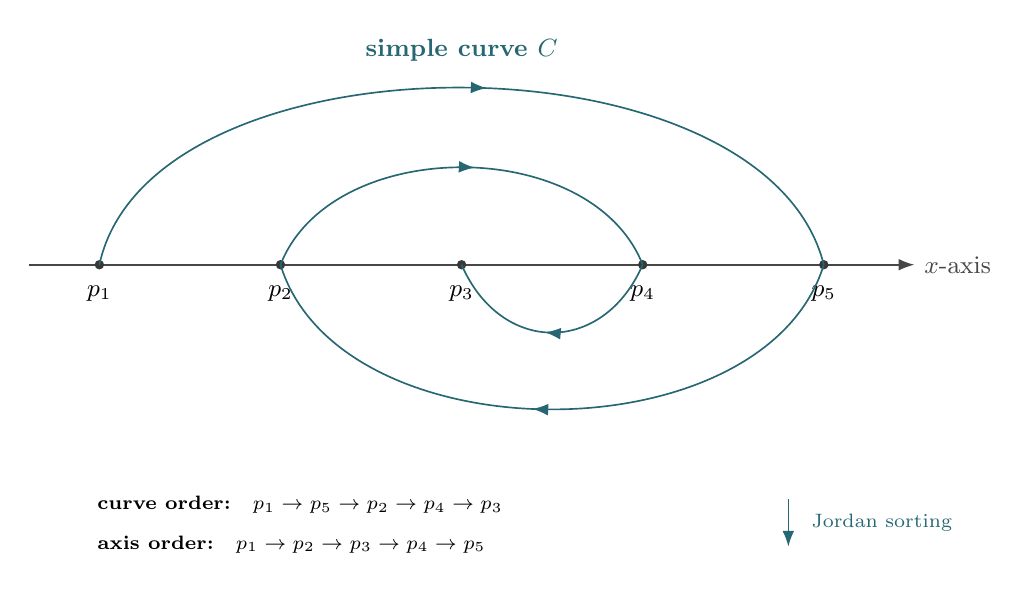
\begin{tikzpicture}[x=1cm,y=1cm,font=\small]
  \coordinate (p1) at (0.8,0);
  \coordinate (p2) at (3.1,0);
  \coordinate (p3) at (5.4,0);
  \coordinate (p4) at (7.7,0);
  \coordinate (p5) at (10.0,0);

  \draw[black!72,semithick,-Latex] (-0.1,0) -- (11.15,0)
    node[right,font=\small] {$x$-axis};

  \foreach \p/\name in {p1/$p_1$,p2/$p_2$,p3/$p_3$,p4/$p_4$,p5/$p_5$} {
    \fill[black!78] (\p) circle (1.7pt);
    \node[below=4pt] at (\p) {\name};
  }

  \tikzset{curve/.style={
    semithick,
    draw=accent,
    postaction={decorate},
    decoration={markings,mark=at position .53 with {\arrow{Latex}}}
  }}
  \draw[curve] (p1) .. controls (1.45,3.0) and (9.25,3.0) .. (p5);
  \draw[curve] (p5) .. controls (9.25,-2.45) and (3.85,-2.45) .. (p2);
  \draw[curve] (p2) .. controls (3.75,1.65) and (7.05,1.65) .. (p4);
  \draw[curve] (p4) .. controls (7.2,-1.15) and (5.9,-1.15) .. (p3);

  \node[accent,text=accent,font=\small\bfseries] at (5.4,2.72) {simple curve $C$};
  \node[font=\scriptsize,align=left,anchor=west] at (0.65,-3.05) {
    \textbf{curve order:}\quad
    $p_1 \rightarrow p_5 \rightarrow p_2 \rightarrow p_4 \rightarrow p_3$
  };
  \node[font=\scriptsize,align=left,anchor=west] at (0.65,-3.55) {
    \textbf{axis order:}\quad
    $p_1 \rightarrow p_2 \rightarrow p_3 \rightarrow p_4 \rightarrow p_5$
  };

  \draw[accent flow] (9.55,-2.98) -- (9.55,-3.58);
  \node[font=\scriptsize,text=accent,anchor=west] at (9.72,-3.28)
    {Jordan sorting};
\end{tikzpicture}
\end{document}
}
  \note{In polygon clipping, a boundary traversal encounters crossings in curve order. The clipping edge needs the same points ordered along the axis. Follow the arrows on the curve, then read the axis from left to right. General comparison sorting needs $\Omega(n\log n)$ comparisons in the worst case. A simple curve restricts the permutations that can occur.}
\end{frame}

\begin{frame}{Research questions}
  \term{Correctness}{Can each backend recover every sorted prefix?}
  \term{Runtime}{How do both backends compare with merge sort and quicksort?}
  \term{Cost}{Which operations give linear total work?}
  \note{Assume distinct, comparable coordinates and a certified Jordan input. Can the reconstructed procedure of Fung et al. recover the output from its own state? Compare both implementations on the same inputs, then bring in Python merge sort and quicksort. Finally, ask how far the operation bounds explain what the clock measures.}
\end{frame}

\begin{frame}{Contributions}
  \begin{itemize}\setlength\itemsep{2.5mm}
    \item Specified $z_1$ corrections, output anchors and exact grouping.
    \item Two backends recover prefixes from their own state.
    \item Paired timings on \UnifiedN{} inputs and growth against general-purpose sorts.
    \item Finite-parent locality and a linear red--black cost bound.
  \end{itemize}
  \note{The reconstruction makes the first-point rules, output position and grouping precise. Both executable backends maintain their own state. A paired experiment on \UnifiedN{} inputs compares the backends, and a supplementary session compares growth with general-purpose sorts. The proof handles finite-parent re-entry and connects the implemented red--black representation to its linear total-work bound.}
\end{frame}

\begin{frame}{Why same-side intervals nest}
  \stateview{\walkDiagram{0}}{Alternating arcs form two families. Within each, intervals are disjoint or nested.}
  \note{Each arc joins consecutive crossings. With the first arc above the axis, even end indices belong to the upper family and odd end indices to the lower family. Trace the nested lower arcs. Interleaved endpoints on the same side would force two arcs to intersect. Each arc's smallest enclosing same-side arc is its parent. The outermost arcs share a dummy root.}
\end{frame}

\begin{frame}{What must survive each insertion?}
  % Owner and children from fig:implementation-family-sibling-structure (a,b).
  \centering
  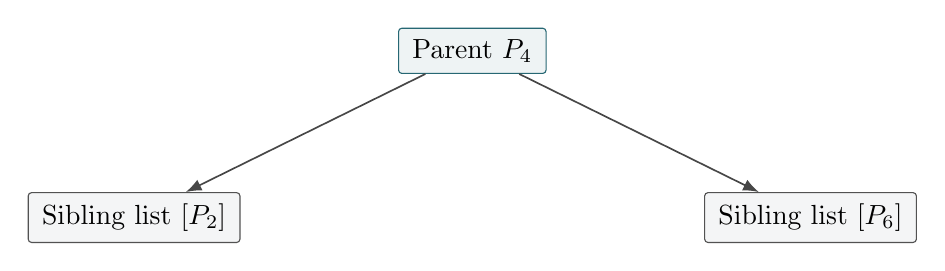
\begin{tikzpicture}[node distance=15mm and 20mm]
    \node[accent box] (p) {Parent $P_4$};
    \node[box,below left=of p] (a) {Sibling list $[P_2]$};
    \node[box,below right=of p] (b) {Sibling list $[P_6]$};
    \draw[flow] (p)--(a); \draw[flow] (p)--(b);
  \end{tikzpicture}
  \captionline{$S_k=\operatorname{sort}(z_1,\ldots,z_k)$}
  One owner per child. A latest child's endpoint determines the cut.
  \note{The prefix list contains exactly the processed points in increasing order. The family trees encode enclosure. Follow the arrows from the parent to its ordered groups of direct children. If the parent is the latest finite member, all its children form one group when nonempty. Otherwise the latest child's last crossing defines the cut into at most two nonempty groups.}
\end{frame}

\begin{frame}{Step 1. Find the predecessor-side boundary}
  \only<1>{\stateview{\walkDiagram{0}}{Find the previous crossing in the sorted prefix.}}
  \only<2>{\stateview{\walkDiagram{1}}{The predecessor leads to the incident upper pair $A_i$.}}
  \note<1>{Read the row of axis values and the row of curve indices separately. The final crossing is still pending. Its pair will belong to the upper family. Start at the previous crossing, which is already in the prefix.}
  \note<2>{Move one position left in that prefix. Follow the predecessor's incident upper arc. This is the insertion-side boundary. Keep it marked while we search in the opposite direction.}
\end{frame}

\begin{frame}{Step 2. Which sibling list can split?}
  \only<1>{\stateview{\walkDiagram{1}}{Return to the previous crossing.}}
  \only<2>{\stateview{\walkDiagram{2}}{The successor selects $B_i$, the first pair in the candidate list.}}
  \only<3>{\stateview{\walkDiagram{2}}{The dashed arc excludes the previous point. Split at the pending value.}}
  \note<1>{Begin again at the old crossing, this time looking to the right in the sorted prefix.}
  \note<2>{The immediate successor is the left endpoint of the dashed upper arc. Following that incidence finds the first pair of the sibling list that may have to split. Parity tells us which incident arc to use.}
  \note<3>{Ask whether the dashed boundary encloses the previous point. If it did, the new pair would acquire no children. Here the previous point is outside. The successor selected the candidate list. The pending value determines where to partition it.}
\end{frame}

\begin{frame}{Step 3(a--b). Insert and split}
  \only<1>{\stateview{\walkDiagram{3}}{At the dummy root: $[P_2]\longrightarrow[P_2,N]$.}}
  \only<2>{\stateview{\walkDiagram{4}}{$[P_6,P_4]\longrightarrow[P_6]\mid[P_4]$. The left group moves under $N$.}}
  \only<3>{\stateview{\walkDiagram{4}}{$N$ owns $[P_6]$. The dummy retains $[P_4]$.}}
  \note<1>{Follow the predecessor-side pair first. It does not enclose the previous crossing. Append the new pair at the end of its sibling list. It inherits the dummy as its parent.}
  \note<2>{Turn to the list beginning at the dashed successor-side pair. Cut at the pending coordinate. An old pair straddling this cut would cross the new arc. The left group lies wholly inside the new interval and becomes its child list.}
  \note<3>{Trace the upper arc to the right of the cut. It remains with the old owner. Check the endpoints against the new arc. The split conserves both old pairs, assigns each one owner and preserves their left-to-right order.}
\end{frame}

\begin{frame}{Step 3(c). Insert at the geometric anchor}
  \only<1>{\stateview{\walkDiagram{5}}{Use the right endpoint of the rightmost child.}}
  \only<2>{\stateview{\walkDiagram{6}}{Insert after the anchor. The prefix is sorted again.}}
  \note<1>{Follow the new pair to its rightmost child, the dashed arc. Read its geometric right endpoint directly from the axis. With no children, the previous crossing would supply the base anchor.}
  \note<2>{The arrow now links the anchor and the pending coordinate. Insert the point immediately after the anchor in the maintained list. Read the completed prefix from left to right.}
\end{frame}

\begin{frame}{Why skip $z_1$ and then use it as the anchor?}
  \only<1>{\stateview{\firstDiagram{1}}{The square marks $z_1$. It has no incident lower pair.}}
  \only<2>{\stateview{\firstDiagram{2}}{Skip $z_1$ during boundary search. The enclosing boundary makes a split unnecessary.}}
  \only<3>{\stateview{\firstDiagram{3}}{Insert after $z_1$ because it lies between the base anchor and the pending value.}}
  \note<1>{Switch to this odd iteration. The previous crossing has the square as its successor. The square is the first crossing of the curve and has only an upper incident pair.}
  \note<2>{Continue to the next successor. Its incident lower pair encloses the previous point. The new pair becomes its child without a split and acquires no children of its own. Its base output anchor is therefore the previous point.}
  \note<3>{Inserting at that base anchor would place the new value before the square, reversing their axis order. Test the output anchor separately. On this odd iteration the square lies strictly between the base anchor and the new value, so insert immediately after the square.}
\end{frame}

\begin{frame}{What a sibling split costs}
  % Condensed fig:proof-split-flow, thesis/figures/source/heterogeneous_split_flow.tex.
  \term{Python lists}{Scan, copy and rebind the transferred pairs.}
  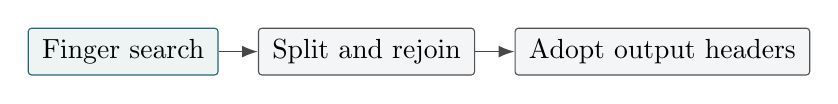
\begin{tikzpicture}[node distance=6mm and 5mm]
    \node[accent box] (s) {Finger search};
    \node[box,right=of s] (p) {Split and rejoin};
    \node[box,right=of p] (a) {Adopt output headers};
    \draw[flow] (s)--(p); \draw[flow] (p)--(a);
  \end{tikzpicture}
  \captionline{Tree split cost grows logarithmically with the smaller side.}
  \note{Recall the newly enclosed child list. Ordinary lists scan and partition the input, materialize outputs and rebind ownership. Even end insertion copies existing IDs. On increasing inputs that copying alone can be quadratic. The red--black tree keeps endpoint fingers and stable handles. It splits along local paths and changes ownership through headers. Endpoint insertion has constant amortized cost. The smaller-side split bound includes a constant term even when one side is empty.}
\end{frame}

\begin{frame}{What does “uninstrumented” remove?}
  \term{Before timing}{Generate ordinary field accesses. Remove observation wrappers.}
  \term{Inside each sort}{Construct the backend, bind methods, sort, recover output.}
  \term{After timing}{Check the output.}
  \note{Both timed backends use minimal execution, disabling traces, selected counters and full post-split validation. Disabling detailed counting in the instrumented tree still intercepts field accesses. Generating the uninstrumented tree removes that machinery while retaining local algorithmic checks. Generation and compilation happen before timing. Per-instance method binding stays inside. Qualification compares both tree configurations on the registered inputs.}
\end{frame}

\begin{frame}{Paired timing on \UnifiedN{} certified inputs}
  % Shortened from fig:method-formal-pipeline, current_experiment_pipeline.tex.
  \centering
  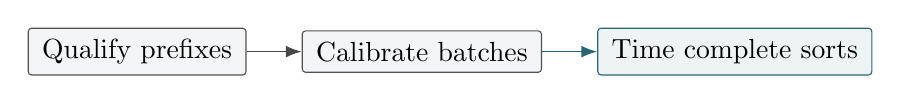
\begin{tikzpicture}[node distance=6mm and 7mm]
    \node[box] (q) {Qualify prefixes};
    \node[box,right=of q] (c) {Calibrate batches};
    \node[accent box,right=of c] (t) {Time complete sorts};
    \draw[flow] (q)--(c); \draw[accent flow] (c)--(t);
  \end{tikzpicture}
  \captionline{\UnifiedWarmups{} warm-ups, \UnifiedRounds{} measured batches per backend and input}
  \vspace{2mm}
  $r_i=\dfrac{\text{median tree time on input }i}{\text{median list time on input }i}$
  \note{The \UnifiedN{} inputs come from common, targeted, structural, geometric and seeded sources. Before timing, compare the states after each prefix and verify outputs. Choose a common batch size for the backends on each input. Alternate first position over the \UnifiedRounds{} measured batches. All saved outputs in the completed formal attempt passed. Each input contributes a single ratio. A value below unity favors the tree.}
\end{frame}

\begin{frame}{The tree/list gap narrows with length}
  \centering\plotfigure{unified_ratio_by_n.pdf}{.60\paperheight}
  \captionline{Pooled band medians\qquad $\UnifiedSmallBandMedian\;\longrightarrow\;\UnifiedLargeBandMedian$}
  \note{The pooled tree/list median falls from \UnifiedSmallBandMedian{} to \UnifiedLargeBandMedian{}. Each plotted line connects exact-length medians within a source. The source mix changes across pooled bands, so the decline alone cannot establish a crossover.}
\end{frame}

\begin{frame}{Heavy nesting favors the finger tree}
  \centering\plotfigure{unified_common_nesting_by_length.pdf}{.55\paperheight}
  \captionline{Tree faster on \UnifiedHeavyWins{} of \UnifiedHeavyN{} heavy inputs. None had a two-sided split.}
  \note{Follow the heavy category across measured even lengths in the common source. Its median falls most sharply. The tree wins on \UnifiedHeavyWins{} of \UnifiedHeavyN{} heavy inputs, each with at most one split. The ordinary backend walks the owner's parent chain and scans sibling lists in liveness checks. Deeper nesting makes that a candidate cost. These complete-sort timings cannot isolate its contribution.}
\end{frame}

\begin{frame}{How fast do the sorting times grow?}
  \centering\plotfigure{baseline_growth.pdf}{.58\paperheight}
  \captionline{Python merge sort and quicksort still finished sooner on every input.}
  \note{The supplementary session timed all methods on the same \BaselineInputs{} inputs. Both Python baselines beat both Jordan backends on every input. For growth, the post hoc subset keeps \BaselineCommon{} common and \BaselineGeometric{} geometric inputs per band. Normalize each method to its own first-band median. First-to-last factors are \BaselineTreeGrowth{} for the tree, \BaselineMergeGrowth{} for merge sort, \BaselineQuickGrowth{} for quicksort, \BaselineListGrowth{} for lists and \BaselineBuiltinGrowth{} for the built-in sort. The tree's adjacent-band exponents span \BaselineTreeMin{} to \BaselineTreeMax{}. These are measured growth factors over this range.}
\end{frame}

\begin{frame}{What the implementation proof adds}
  % Three-row abridgement of tab:proof-relation, thesis/appendix/backend_argument.tex.
  \renewcommand{\arraystretch}{1.50}
  \begin{tabular}{@{}>{\raggedright\arraybackslash}p{.25\linewidth}>{\raggedright\arraybackslash}p{.27\linewidth}>{\raggedright\arraybackslash}p{.39\linewidth}@{}}
    \toprule
    & \textbf{Fung et al.} & \textbf{This thesis}\\
    \midrule
    Locality & Latest child & Finite-parent re-entry\\
    Representation and operations & Upward ribs & Red--black repairs, mixed updates\\
    Total cost & List-size potential & Core, ownership, output in $O(n)$\\
    \bottomrule
  \end{tabular}
  \note{Fung et al. prove locality when a child is latest and mention the finite-parent case. The thesis proves that re-entry case and uses exact grouping and ownership in the prefix induction. The paper sketches upward ribs. Here the red--black representation is decoded and preserved by insert, join and split. A node potential pays for repairs across mixed updates. The paper's list-size potential then pays all smaller-side split charges. Including core, ownership and output gives linear expected/amortized work for the minimal tree under unit-cost comparisons and word operations, expected dictionary lookup and amortized growth.}
\end{frame}

\begin{frame}{Conclusions and limits}
  \term{Correctness}{Both backends maintain sorted prefixes.}
  \term{Cost}{The finger tree realizes linear expected/amortized work.}
  \term{Runtime}{Tree faster on \UnifiedWins{} of \UnifiedN{} inputs.}
  \captionline{Does the gap keep narrowing beyond $n=\UnifiedMaxN$?}
  \note{The reconstruction specifies the split list, transferred group and geometric anchor. The cost argument applies to the implemented tree in its stated model. The overall median tree/list ratio was \UnifiedMedian{}. Heavy nesting produced its strongest measured advantages, and its time grew more slowly than the Python baselines over this range. Measurements stop at length \UnifiedMaxN{} on a single CPython host with certified valid inputs. Larger application-derived inputs and targeted parent-chain measurements would test the trend and its cause.}
\end{frame}

\begin{frame}[plain]\relax
  \centering{\Huge\bfseries Questions?}
  \note{Invite questions. The backup pages cover the reflected first-point correction, absolute timings, comparison counts, locality, amortization and qualification.}
\end{frame}

\appendix
\setbeamertemplate{footline}{}

\begin{frame}[noframenumbering]{The reflected $z_1$ correction}
  \centering% Adapted from thesis/figures/source/step3c_anchor_z1_anomaly.tex.
\newcommand{\ordernode}[5][]{%
  \node[box,minimum width=1.12cm,minimum height=.76cm,#1] (#2) at (#3) {#4\\[-2pt]\scriptsize #5};%
}

\begin{tikzpicture}[font=\small]
  \node[anchor=east] at (1.02,2.18) {Before};
  \foreach \label/\value [count=\i] in {z_1/1,z_2/2,z_3/3,z_4/4,z_5/6,z_6/7} {
    \ordernode{a\i}{1.0+1.38*\i,2.18}{$\label$}{$\value$}
    \ifnum\i>1
      \draw[flow] (a\the\numexpr\i-1\relax.east) -- (a\i.west);
    \fi
  }
  \draw[accent,thick] ($(a2.north west)+(0,.12)$)--($(a2.north east)+(0,.12)$)
      node[midway,above]{base anchor};
  \node[anchor=east] at (1.02,-.17) {After};
  \foreach \label/\value [count=\i] in {z_7/0,z_1/1,z_2/2,z_3/3,z_4/4,z_5/6,z_6/7} {
    \ifnum\i=1
      \ordernode[draw=accent,fill=accent!8,minimum width=1.02cm]
        {b\i}{.40+1.31*\i,-.17}{$\label$}{$\value$}
    \else
      \ordernode[minimum width=1.02cm]
        {b\i}{.40+1.31*\i,-.17}{$\label$}{$\value$}
    \fi
    \ifnum\i>1
      \draw[flow] (b\the\numexpr\i-1\relax.east) -- (b\i.west);
    \fi
  }
  \draw[accent,thick] ($(b2.north west)+(0,.12)$)--($(b2.north east)+(0,.12)$)
      node[midway,above]{corrected anchor};
\end{tikzpicture}

  \captionline{On this odd step, $z_i<z_1<a_i$. Insert before $z_1$.}
  \note{The reflected step acquires the right split side and uses the left endpoint of the leftmost child when present. In the decreasing counterexample from the thesis, the incoming value is the new minimum. Its geometric base anchor lies to the right of the first crossing. Inserting immediately before the base anchor would leave that first crossing on the wrong side. The strict between-test moves the anchor to the first crossing. This is separate from skipping the first point during the lower-family search.}
\end{frame}

\begin{frame}[noframenumbering]{Absolute time per sort}
  \centering\plotfigure{baseline_runtime.pdf}{.66\paperheight}
  \note{Read the vertical axis in microseconds per complete sort on a logarithmic scale. The supplementary session interleaved both Jordan backends, the Python baselines and the built-in sort. The median paired tree/merge and tree/quick time ratios were \BaselineTreeMerge{} and \BaselineTreeQuick{}. These are within-input ratios.}
\end{frame}

\begin{frame}[noframenumbering]{Key comparisons per element}
  \centering\plotfigure{baseline_comparisons.pdf}{.62\paperheight}
  \captionline{On \BaselineTreeFewerQuick{} inputs, the tree made fewer comparisons than quicksort and still took longer.}
  \note{The separate untimed pass wraps keys and counts executed order comparisons, including those with numeric sentinels. Equality tests and hashing are excluded. The tree used more comparisons than merge sort on every input and more than quicksort on \BaselineTreeMoreQuick{}. Counts alone cannot account for the timings.}
\end{frame}

\begin{frame}[noframenumbering]{Finite-parent re-entry and exact grouping}
  \term{Hypothesis}{The finite parent is latest. Its region stays unchanged.}
  \term{First re-entry}{Use the gap immediately inward from its latest endpoint.}
  \note{Let the gap run from the parent's latest endpoint to the nearest child endpoint inward, or to the other parent endpoint when it has no child. A re-entry beyond that gap would give a crosscut which, together with the later curve portion, separates boundary points that the older simple curve still connects. The contradiction forces the inward gap and supports the exact grouping invariant.}
\end{frame}

\begin{frame}[noframenumbering]{How the two potentials pay for a run}
  \term{Node potential}{Pays for red--black repair propagation across mixed insertions and splits.}
  \term{List-size potential}{Pays the smaller-side split charges over the whole run.}
  \note{The local argument gives constant amortized endpoint insertion and logarithmic-in-the-smaller-side amortized splitting. Applying the list-size potential across the legal operation history pays those split terms in aggregate. Bounded header updates and shared-core work preserve the linear expected/amortized total under the stated model.}
\end{frame}

\begin{frame}[noframenumbering]{Qualification and the timing boundary}
  \term{Before}{Check tree equivalence, prefix states, replay and minimal output.}
  \term{Timed}{Initialize, bind methods, sort, recover and collect output.}
  \term{After}{Verify saved outputs and recompute summaries.}
  \note{Checked instances advance through corresponding prefixes. Fresh checked replay and a fresh minimal call provide further checks. Expected answers are computed outside the sorting core. Explicit pre-batch collection precedes the interval, while automatic garbage collection stays enabled. Per-instance tree setup stays in the reported times. Archive validation independently checks outputs and summaries.}
\end{frame}
\end{document}
